
%% Beamer poster theme created for Imperial College by LianTze Lim
%% LICENSE: LPPL 1.3
\documentclass[xcolor={table}]{beamer}
\usepackage[size=a0,orientation=landscape,scale=1.55]{beamerposter}
\setlength{\oddsidemargin}{1in}
\usepackage{wrapfig}
\usepackage{amsmath}
\usepackage{tabu}
\usepackage{booktabs}
%\usepackage{subcaption}
\usepackage[caption=false]{subfig}
% \captionsetup[table]{font={stretch=1.2}}     %% change 1.2 as you like

\newcommand{\arxiv}[1]{}  % bib was designed for stupid natbib
\newcommand{\httpsurl}[1]{\href{https://#1}{\nolinkurl{#1}}}

\usetheme{ImperialPoster}
%% Four available colour themes
\usecolortheme{ImperialWhite} % Default
% \usecolortheme{ImperialLightBlue}
% \usecolortheme{ImperialDarkBlue}
% \usecolortheme{ImperialBlack}

\title{Demystifying MMD GANs}
\author{
  \mainauthor{Miko{\l}aj Bi\'nkowski}\Tsup{1} \quad
  \mainauthor{Dougal J. Sutherland}\Tsup{2} \quad
  Michael Arbel\Tsup{2} \quad
  Arthur Gretton\Tsup{2}
}
\institute{
  \Tsup{1}Department of Mathematics, Imperial College London \quad
  \Tsup{2}Gatsby Computational Neuroscience Unit, University College London\\
  \texttt{\{mikbinkowski,dougal,michael.n.arbel,arthur.gretton\}@gmail.com}
}

\DeclareMathOperator{\D}{\mathcal{D}}
\DeclareMathOperator*{\E}{\mathbb{E}}
\newcommand{\F}{\mathcal{F}}
\newcommand{\h}{\mathcal{H}}
\DeclareMathOperator{\mean}{mean}
\newcommand{\PP}{\mathbb P}
\newcommand{\QQ}{\mathbb Q}
\newcommand{\R}{\mathbb R}
\DeclareMathOperator{\W}{\mathcal{W}}
\newcommand{\X}{\mathcal X}
\newcommand{\Z}{\mathcal Z}
\newcommand{\ZZ}{\mathbb Z}
\DeclareMathOperator*{\argmin}{argmin}
\DeclareMathOperator*{\argmax}{argmax}
\DeclareMathOperator{\mmd}{MMD}
\DeclareMathOperator{\FID}{FID}

\addbibresource{refs.bib}

\definecolor{blackish}{RGB}{16,14,12}

\begin{document}
\addtobeamertemplate{headline}{} % Imperial Logo. This is a bit hacky
{
\begin{tikzpicture}[remember picture,overlay]
\node (uclbox) [shift={(-.39\linewidth,-3.25cm)}, align=left] at (current page.north east) {
  
\includegraphics[height=13cm]{UCL_Black_Landscape.pdf} };

\draw[fill=blackish](current page.north west) rectangle ([yshift=.2225cm, xshift=2cm] uclbox.south west);

\node[shift={(8.5cm,-6.5cm)}] at (current page.north west) { 
\includegraphics[height=3.5cm]{Imperial_logo_white.pdf}};
\end{tikzpicture}
% \begin{tikzpicture}[remember picture,overlay]
% \node[shift={(-10cm,-5cm)}] at (current page.north east) { 
\includegraphics[height=7cm]{gatsby.jpg}};
% \end{tikzpicture}
}

\begin{frame}{}
\maketitle
\begin{columns}[T, totalwidth=\textwidth]

  \begin{column}{.32\textwidth}
    % TODO: fiddle with spacing in alertblock
    \begin{alertblock}{\;Overview}
      \begin{itemize}\raggedright
        \item MMD GANs are related to WGANs, but with part of critic function optimization done in closed form.
        \item Outperform WGAN-GP, especially with smaller critic network.
        \item Clarify gradient bias situation:
              ``outer loop'' generator gradients are biased,
              but each step is unbiased.
        \item New GAN performance metric, KID, with better estimator than FID;
              use it to adapt the learning rate during training.
      \end{itemize}
    \end{alertblock}
    % \vspace*{-1.2cm}
    \begin{block}{Relation to Wasserstein and Cram\'er GANs}
      Integral Probablity Metrics (IPMs) %form a family of divergences between
      are distances between distributions
      defined by a class of \emph{critic} functions $\F$:
      \[
        \D(\PP, \QQ)
        = \sup_{f \in \F} \D_f(\PP, \QQ)
        = \sup_{f\in\F} \E_{X\sim\PP}[f(X)] - \E_{Y\sim\QQ}[f(Y)].
      \]

      \vspace*{-1.5ex}\begin{itemize}
        \item{\textbf{Wasserstein distance} has $\F$ the set of 1-Lipschitz functions
          \[
            \F = \left\{f: \sup_{x,y} \frac{|f(x) - f(y)|}{\|x - y\|}\leq 1\right\}.
          \]
          WGANs approximate $f$ with a critic network,
          made approximately Lipschitz with
          weight clipping \parencite{wgan}
          or gradient penalty \parencite{wgan-gp}.
        \item \textbf{Maximum Mean Discrepancy (MMD)} %\parencite{mmd-jmlr}
          has $\F$ a unit ball in a
          \emph{Reproducing Kernel Hilbert Space (RKHS)} $\h$ with kernel $k$: % \\
          % \textbf{\color{red} TODO: dogs and fish}
          % \[ \F = \left\{f: \|f\|_{\h} \leq 1\right\}. \]
          % MMD value and the optimal critic are known in closed form:
          \begin{minipage}{.49\linewidth}
            \begin{gather*}
              f^*(t) \propto \E_{\PP}k(X, t) - \E_{\QQ}k(Y, t)
              \\
              \mmd_k^2:
            \end{gather*}
          \end{minipage}
          \begin{minipage}{.49\linewidth}
          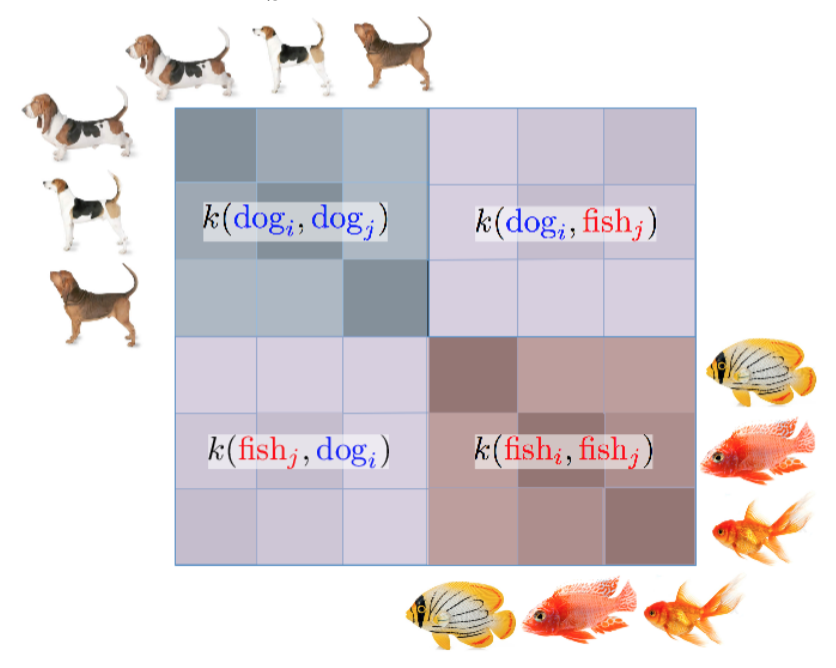
\includegraphics[width=\linewidth]{figs/dogfish.png}
          \end{minipage}
          % \begin{align*}
            % \mmd_k^2(\PP, \QQ) &= \E_{\PP} k(X,X') + \E_{\QQ} k(Y,Y') - 2\E_{\PP,\QQ} k(X,Y),\\
            % f^*(t) &\propto \E_{\PP}k(X, t) - \E_{\QQ}k(Y, t).
          % \end{align*}
        }
        \item
          MMD GANs \parencite{mmd-gan} optimize \emph{representation} in kernel
          \[ k_{\theta}(x, y) = k_\mathrm{base}(h_{\theta}(x), h_{\theta}(y)), \]
          corresponding to distance
          \[ \D(\PP, \QQ) = {\sup}_\theta \D_\theta(\PP, \QQ) = {\sup}_{\theta} \mmd_{k_\theta}^2(\PP, \QQ). \]
        \item Cram\'er GAN \parencite{cramer-gan} almost same, with \emph{Energy Distance} $k_\mathrm{base}$.
        % \item WGANs are \emph{almost} an MMD GAN with linear $k_\mathrm{base}$.
      \end{itemize}
    \end{block}

    \begin{block}{MMD GAN with Gradient Penalty}
      Like WGAN-GPs \parencite{wgan-gp}, we penalize
      gradient of the critic function:
      \[ Loss^{critic}(\theta) = \widehat{\mmd}_{\theta}^2(\PP, \QQ_{\psi}) + \lambda\E_{\tilde{X}}\left(\|\nabla_{\tilde{X}} f^*(\tilde{X})\| - 1\right)^2. \]
      %where $\tilde{X}$ are drawn between points from $\PP$ and $\QQ_{\psi}$. %$\widehat{MMD}$ is an unbiased MMD estimator.% and $\QQ_{\psi} = G_{\psi}(\ZZ)$ is the generated distribution.
      With linear $k_\mathrm{base}$,
      \emph{almost} the same as a WGAN-GP.
    \end{block}
  \end{column}

  \begin{column}{.32\textwidth}
    \vspace*{-1cm}
      % Wasserstein and (Gaussian kernel) MMD optimal critics: \\[1ex]
      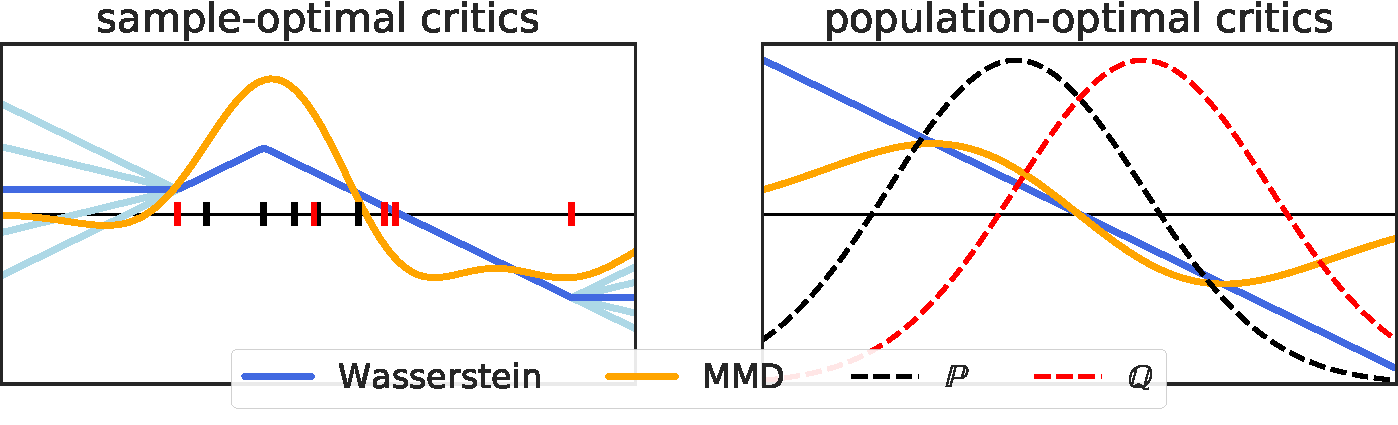
\includegraphics[width=\linewidth]{figs/witness.pdf}
      % Note multiple sample-optimal Wasserstein critics (light blue).

    % \vspace*{-1.3cm}
    \begin{block}{Theory: Biased gradient estimates}
      \textcite{cramer-gan} claim that WGANs have biased generator gradients, while Cram\'er GANs do not. We show:
      \vspace*{-1.5ex}
      \begin{itemize}
        \item For a \emph{fixed} kernel/critic,
              generator gradient steps are unbiased.
              % (Same for critic.)
        % \begin{itemize}
        %   \item General proof of $\E \nabla f = \nabla \E f$ for feedforward networks $f$.
        % \end{itemize}
        \item ``Outer loop'' gradient steps, $\nabla_\psi \hat\D(X, G_{\psi}(Z))$, are biased.
        \begin{itemize}
          \item Estimators with non-constant bias have biased gradients.
          \item Optimization-based estimators are biased:
            \[
            \E \hat\D%(X, Y)
                 = \E \hat\D_{\hat f_{tr}}(X_{te}, Y_{te})
                 = \E \D_{\hat f_{tr}}(\PP, \QQ)
                 \le {\sup}_f \D_f
                 = \D
            .\]
          % \item No possible unbiased estimator exists for IPMs $\D$.
          \item Small minibatch sizes \emph{don't} introduce bias: bias vanishes as critic becomes optimal.
        \end{itemize}
      \end{itemize}
    \end{block}
    \vspace*{-1.5ex}
    \begin{block}{Experimental comparison}
      MMD GANs outperform WGAN-GP, especially with \emph{smaller} critic networks (faster to train),
      probably by ``offloading'' work to closed-form kernel optimization.
%      MMD GANs with gradient penalty and right kernel lead to better results
%      than WGAN-GP and allow limiting the size of the critic
%      network, while preserving sample quality. %We recommend use of a mixture of rational-quadratic kernels.
%      MMD GANs also allow limiting the size of the critic
%      network, while preserving sample quality.
    \end{block}
    \vspace*{-1.3cm}
%    \begin{figure}
%      \centering
%      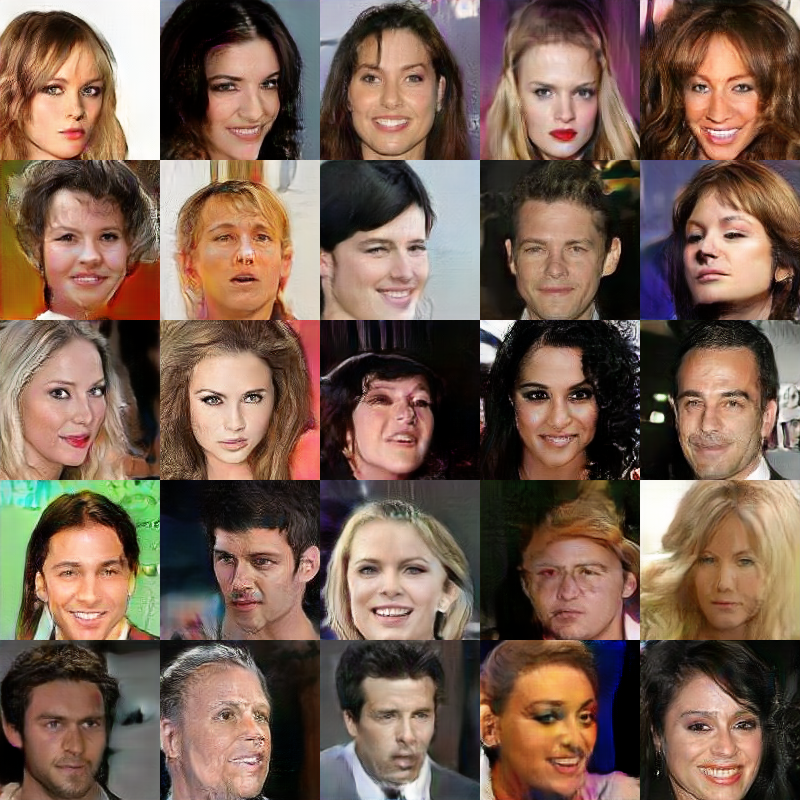
\includegraphics[width=.32\columnwidth]{samples/celeba-mmd-rq-25.png}
%      ~
%      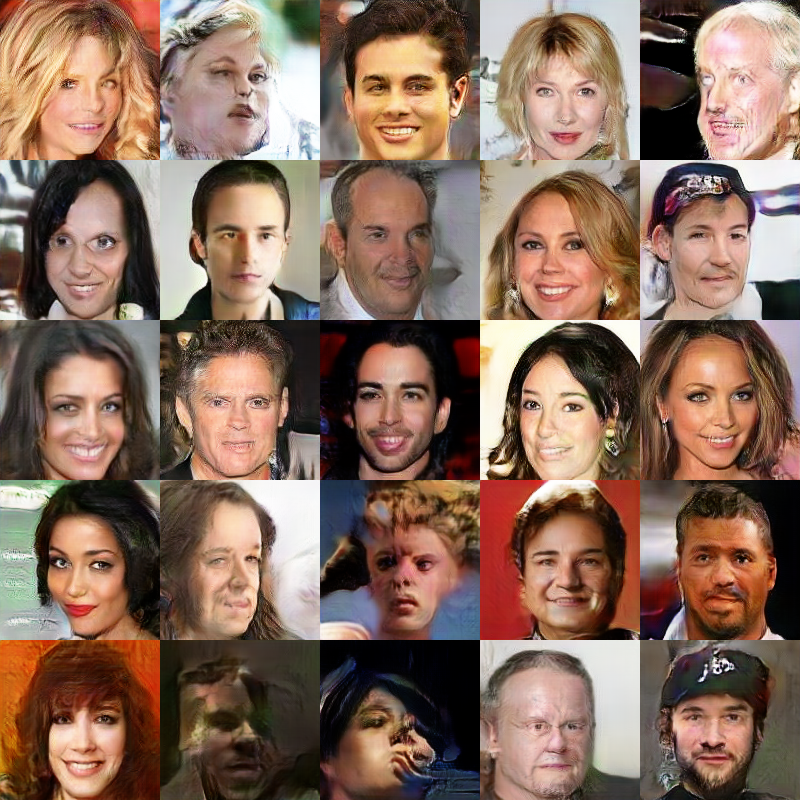
\includegraphics[width=.32\columnwidth]{samples/celeba-wgan-25.png}
%      ~
%      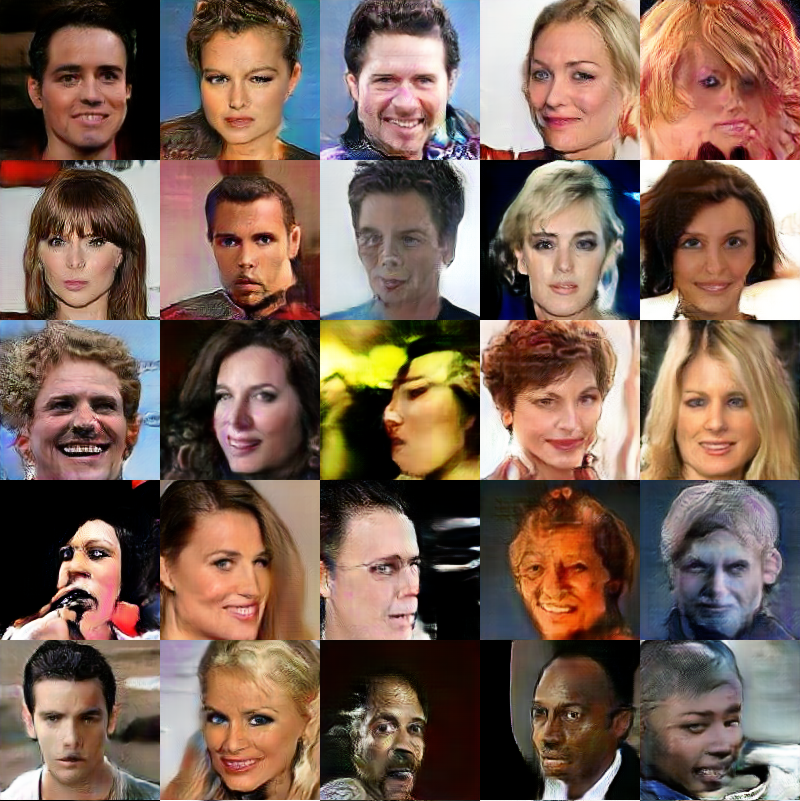
\includegraphics[width=.32\columnwidth]{samples/celeba-cramer-25.png}
%      \caption{Samples for \textbf{$160 \times 160$ CelebA} dataset trained with
%               MMD GAN (left) and WGAN-GP (right) with ResNet generator and DCGAN discriminator.}
%    \end{figure}

    \begin{minipage}{.57\linewidth}
      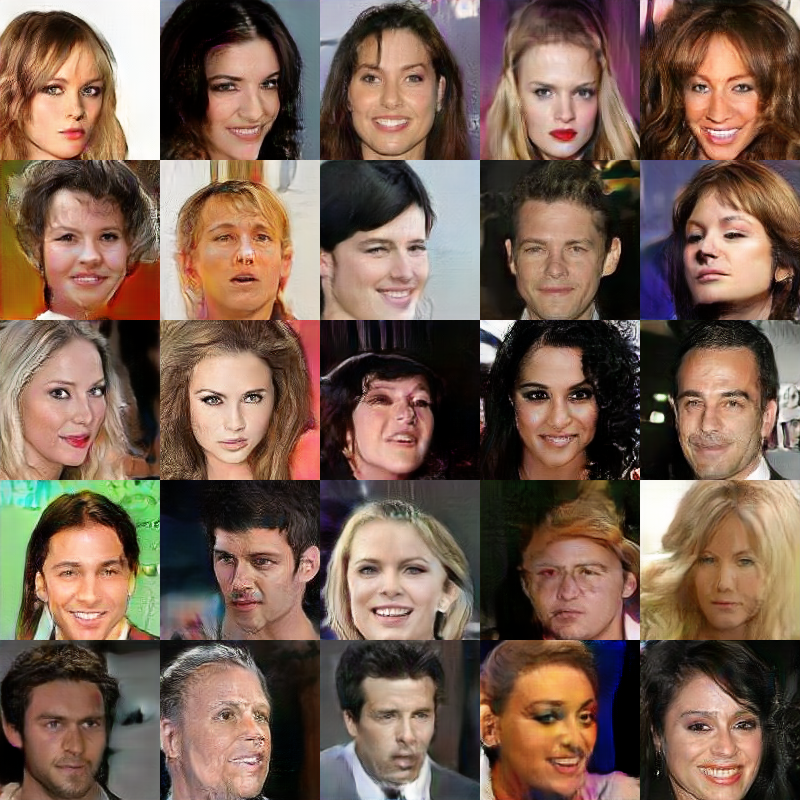
\includegraphics[width=.49\linewidth]{samples/celeba-mmd-rq-25.png}
      \hfill
      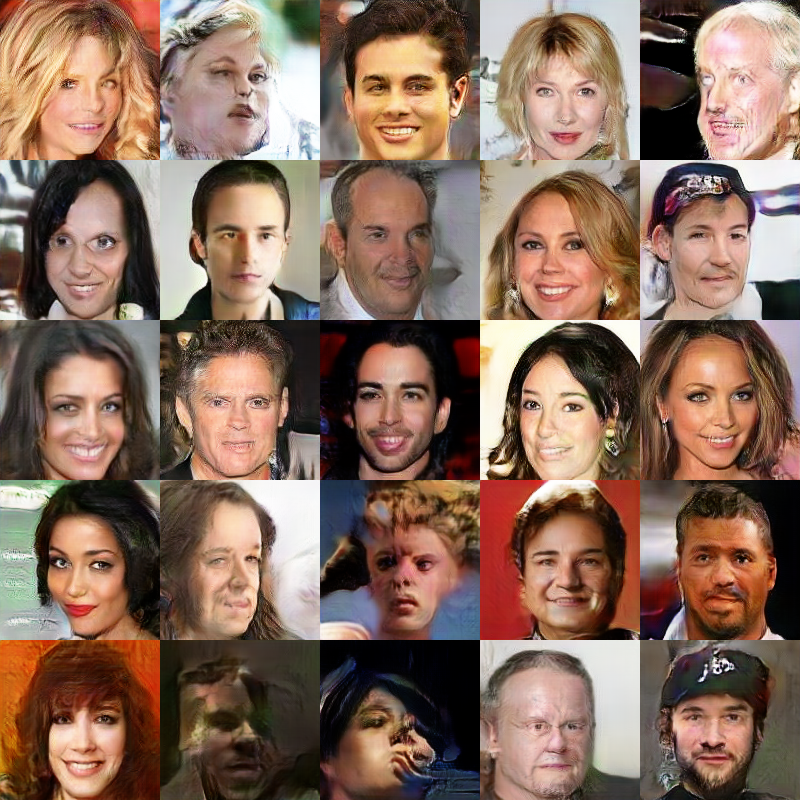
\includegraphics[width=.49\linewidth]{samples/celeba-wgan-25.png}
    \end{minipage}
    \begin{minipage}{.42\linewidth}\raggedright
      \textbf{CelebA, $160 \times 160$.} \\
      MMD GAN (left) and WGAN-GP (right),
      with ResNet generator and DCGAN critic.
    \end{minipage}
    \\[.5ex]

    \begin{minipage}{.57\linewidth}
      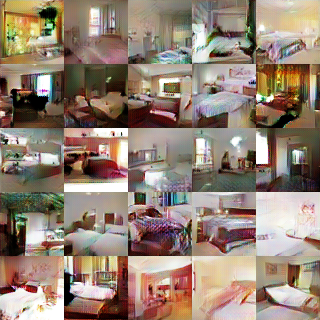
\includegraphics[width=.49\linewidth]{samples/lsun_rq_16.png}
      \hfill
      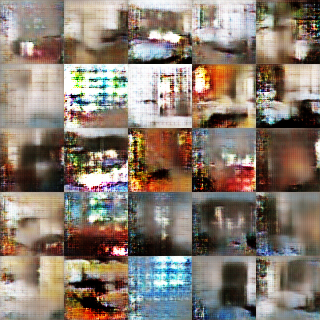
\includegraphics[width=.49\linewidth]{samples/lsun_wgan_16.png}
    \end{minipage}
    \begin{minipage}{.42\linewidth}\raggedright
       \textbf{LSUN bedrooms, $64 \times 64$.}\\
       MMD GAN (left) and WGAN-GP (right),
       with \emph{small critic} DCGANs ($4\times$ less convolutional filters).
    \end{minipage}
    ~\\[1.5ex]

    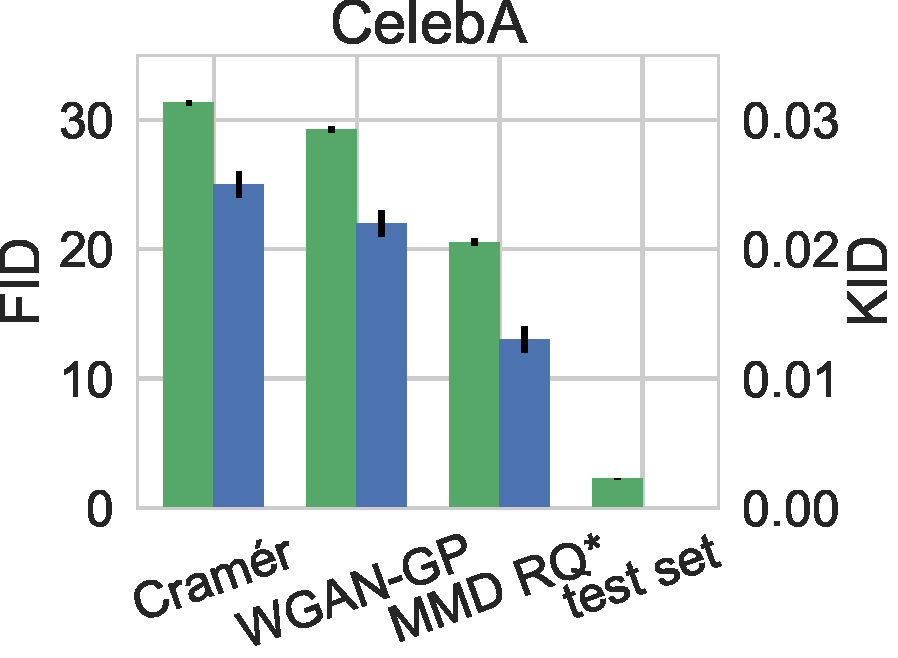
\includegraphics[width=.48\linewidth]{figs/celeba-scores.pdf}
    \hfill
    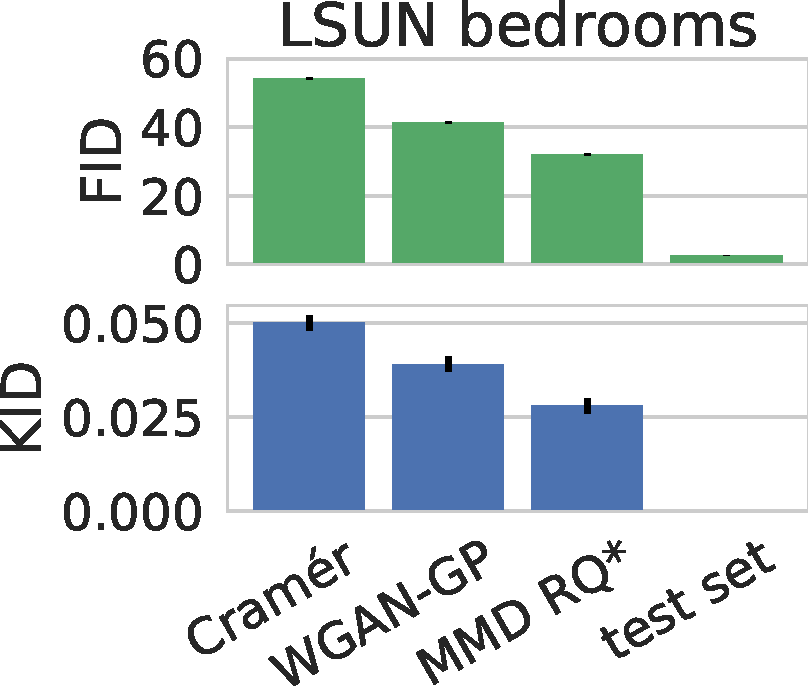
\includegraphics[width=.48\linewidth]{figs/lsun-scores.pdf}

  %   CelebA scores (mean + standard deviation):
  %   % \begin{table}
  %   %   \centering
  %   %   \vspace{-1cm}
  %   %   \caption{Mean (standard deviation) of score evaluations for the CelebA dataset.}
  %   %   \label{tab:celeba-scores}
  %   \begingroup \renewcommand{\arraystretch}{1.1}
  %   \begin{tabular}{cc|rrr}
  %       loss & top layer & \multicolumn{1}{c}{Inception} & \multicolumn{1}{c}{FID} & \multicolumn{1}{c}{KID} \\
  %       \hline
  %       MMD RQ   &   16 &\quad   2.61  (0.01) &\quad \textbf{20.55}  (0.25) &\quad \textbf{0.013}  (0.001)\\
  %       Cram\'er &  256 &    2.86  (0.01) &   31.30  (0.17) &   0.025  (0.001)\\
  %       WGAN-GP  & 1    &\textbf{2.72}  (0.01) &   29.24  (0.22) &   0.022  (0.001)\\
  %       \multicolumn{2}{c|}{test set} &    3.76  (0.02) &    2.25  (0.04) &   0.000  (0.000)\\
  %   \end{tabular}
  %   \endgroup
  % % \end{table}
  \end{column}

  \begin{column}{.32\textwidth}
    \begin{block}{New evaluation method: KID}
      Inception scores aren't meaningful for LSUN or CelebA.

      Fr\'echet Inception Distance (FID) \parencite{fid} better,
      but biased estimator:
      \vspace*{-1.5ex}\begin{itemize}
        \item Estimator has very strong bias, almost no variance.
        \item
        Easy to find $\PP_1$, $\PP_2$, $\QQ$ where for reasonable sample sizes
        \[
          \FID(\PP_1, \QQ) < \FID(\PP_2, \QQ)
          \;\text{ but }\;
          \E \FID(\hat\PP_1, \QQ) > \E \FID(\hat\PP_2, \QQ)
        .\]
        \item Monte Carlo ``confidence intervals'' are meaningless.
      \end{itemize}

      Proposed \emph{Kernel Inception Distance} (KID):
      $\mmd^2$ estimate with kernel $k(x, y) = \left( x^{\mathsf T} y / d + 1 \right)^3$
      between Inception representations.
      \vspace*{-1.5ex}\begin{itemize}
        \item Estimator has no bias, small variance.
        \item Computationally faster, needs fewer samples than FID.
        \item Asymptotically normal: easy Monte Carlo confidence intervals.
      \end{itemize}

      CIFAR-10 train to test estimates, increasing sample sizes:
      % FID has strong bias and almost no variance;
      % KID has no bias and rapidly decreasing variance.
      \\
      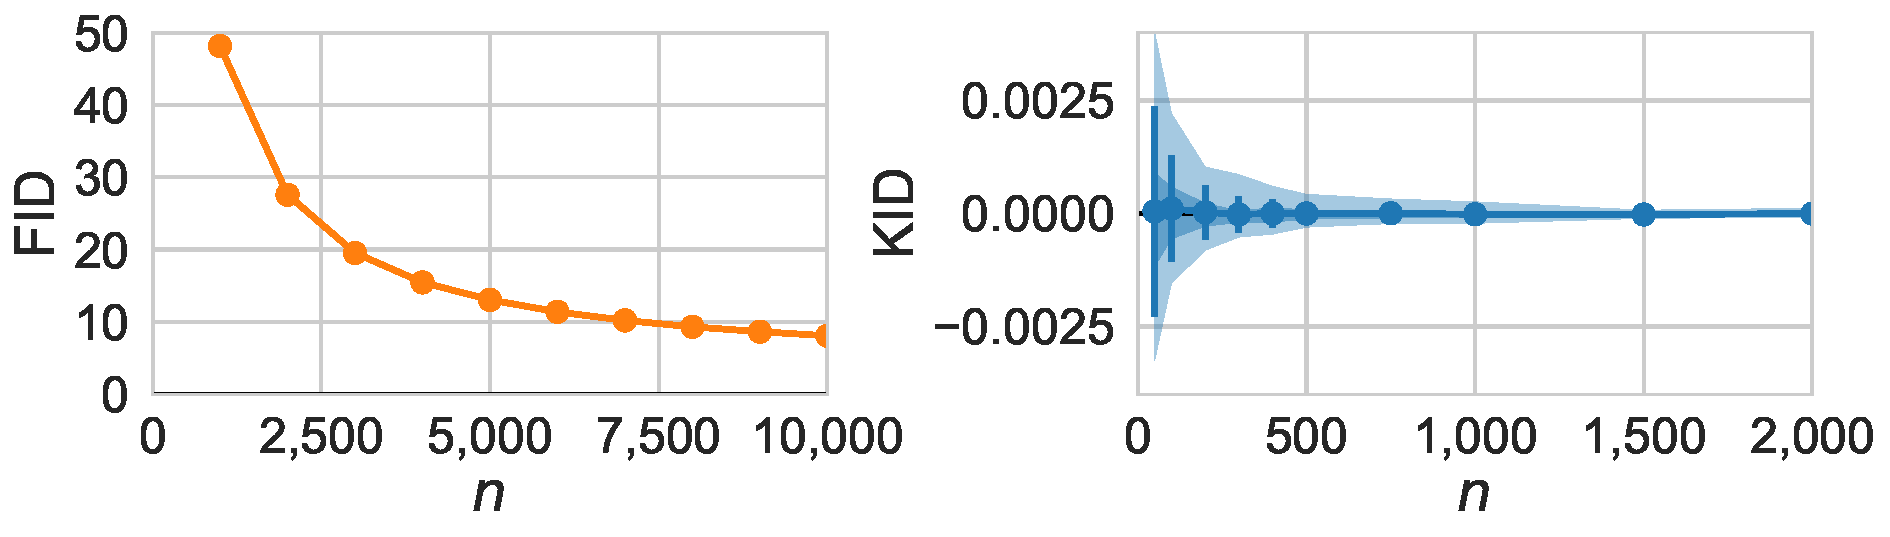
\includegraphics[width=\columnwidth]{figs/fid-kid-bias-comparison.pdf}

        % \caption{Estimates of KID (left) and FID (right) between the CIFAR-10 train and test sets. FID estimates
        %   exhibit strong bias for $n$ even up to $10\,000$, which is not the case for KID.
        %   Standard deviation of estimates shrinks quickly for KID and is always small for FID.}  %Each point is based on 100 samples, estimating with replacement; sampling without replacement, and/or using the full training set, gives similar results. Lines show means, error bars standard deviations, dark colored regions a $\frac{2}{3}$ coverage interval of the samples, light colored regions a $95\%$ interval. Note the differing $n$ axes.}
        % \label{fig:fid-kid-bias}
    \end{block}

    \vspace*{-1cm}
    \begin{block}{Learning Rate Adaptation}
      Automatic learning rate adaptation using 3-sample test \parencite{3sample}:

      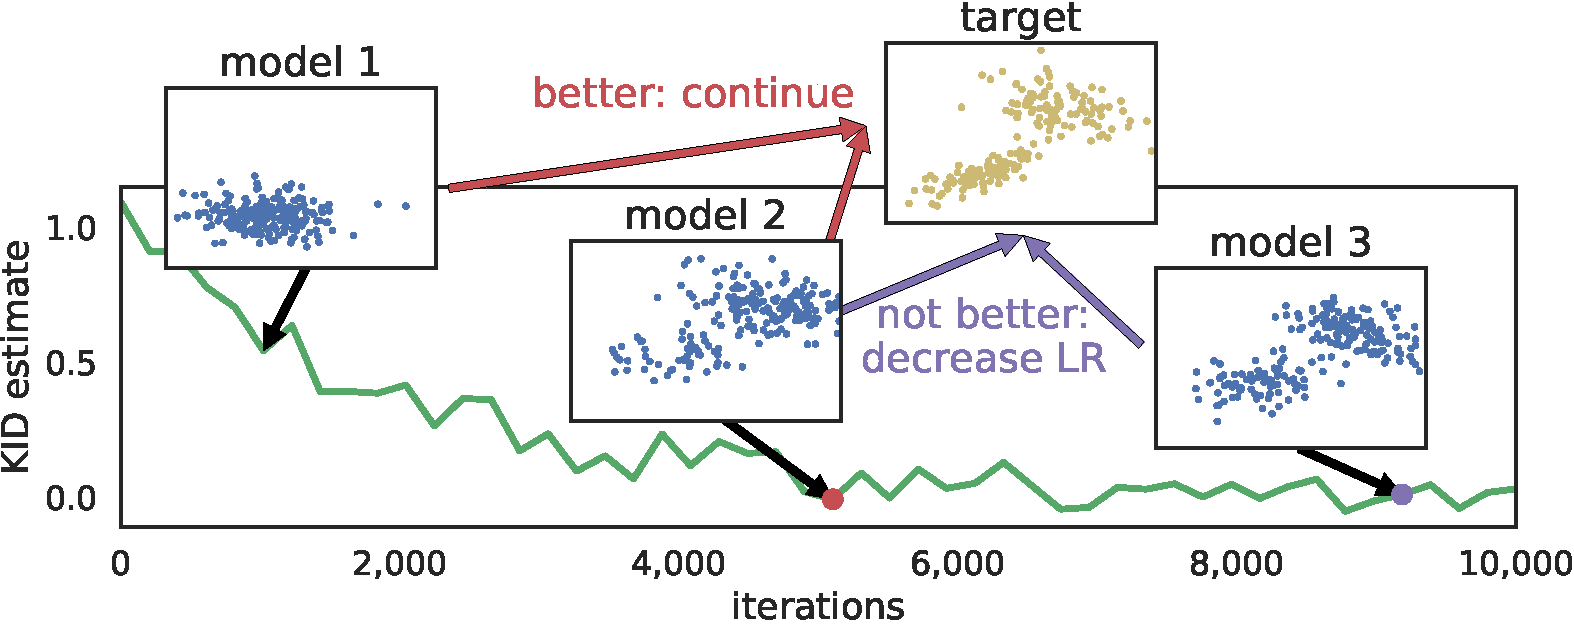
\includegraphics[width=\linewidth]{figs/KID-LR.pdf}
%       \textbf{\color{red} TODO: picture instead}
%       \begin{itemize}
% %        \item Decreasing learning rate is common in deep learning.
%         \item GAN learning rates usually tuned by hand; need to get it right.
%         \item We propose an adaptive scheme: decrease if the KID score hasn't improved for a while, using an \emph{MMD relative similarity test} \parencite{3sample}.
%       \end{itemize}
    \end{block}

    \vspace*{-2ex}
    \begin{block}{Implementation}
      \begin{center}
        {\color{blue} \httpsurl{github.com/mbinkowski/MMD-GAN/}}
      \end{center}
    \end{block}

    \printbibliography
  \end{column}

\end{columns}


\end{frame}


\end{document}
